\documentclass[12pt,a4paper]{article}
\usepackage[utf8]{inputenc}
\usepackage[T1]{fontenc}
\usepackage[margin=2.5cm]{geometry}
\usepackage{graphicx}
\usepackage{hyperref}
\usepackage{enumitem}
\usepackage{xcolor}
\usepackage{tikz}
\usetikzlibrary{shapes.geometric, arrows, positioning}
\usepackage{fancyhdr}
\usepackage{titlesec}

\definecolor{primary}{RGB}{220, 38, 38}
\definecolor{secondary}{RGB}{248, 113, 113}

\hypersetup{
    colorlinks=true,
    linkcolor=primary,
    urlcolor=primary
}

\pagestyle{fancy}
\fancyhf{}
\fancyhead[L]{Software Development Project}
\fancyhead[R]{Lecture 6: SDLC}
\fancyfoot[C]{\thepage}

\title{\textbf{Lecture 6: Software Development Life Cycle (SDLC)}\\[0.5cm]\large Understanding the Complete Development Process}
\author{State University of Zanzibar (SUZA)\\BSc Computer Science}
\date{}

\begin{document}

\maketitle
\tableofcontents
\newpage

\section{Introduction to SDLC}

\subsection{What is SDLC?}
The Software Development Life Cycle (SDLC) is a systematic process for planning, creating, testing, and deploying software applications. It provides a structured framework that ensures:
\begin{itemize}
    \item Quality software is delivered on time
    \item Development costs are controlled
    \item Customer requirements are met
    \item Risks are minimized
\end{itemize}

\subsection{Why is SDLC Important?}
\begin{enumerate}
    \item \textbf{Predictability:} Provides clear milestones and deliverables
    \item \textbf{Quality:} Ensures systematic testing and review
    \item \textbf{Documentation:} Creates comprehensive project records
    \item \textbf{Risk Management:} Identifies problems early
    \item \textbf{Cost Control:} Prevents budget overruns
\end{enumerate}

\section{The Seven Phases of SDLC}

\subsection{Phase 1: Planning}

\textbf{Purpose:} Define the project scope, objectives, and feasibility.

\textbf{Key Activities:}
\begin{itemize}
    \item Define project goals and objectives
    \item Conduct feasibility study (technical, economic, operational)
    \item Identify stakeholders
    \item Create project timeline
    \item Allocate budget and resources
    \item Risk assessment
\end{itemize}

\textbf{Deliverables:}
\begin{itemize}
    \item Project Charter
    \item Feasibility Study Report
    \item Project Plan
    \item Risk Assessment Document
\end{itemize}

\textbf{Example Questions to Answer:}
\begin{enumerate}
    \item What problem are we solving?
    \item Who are the users?
    \item What is the budget and timeline?
    \item Is this project technically feasible?
\end{enumerate}

\subsection{Phase 2: Requirements Analysis}

\textbf{Purpose:} Gather and document detailed requirements.

\textbf{Key Activities:}
\begin{itemize}
    \item Conduct stakeholder interviews
    \item Gather functional requirements (what the system does)
    \item Gather non-functional requirements (performance, security)
    \item Create user stories and use cases
    \item Prioritize requirements (MoSCoW method)
    \item Get stakeholder approval
\end{itemize}

\textbf{Deliverables:}
\begin{itemize}
    \item Software Requirements Specification (SRS)
    \item User Stories
    \item Use Case Diagrams
    \item Requirements Traceability Matrix
\end{itemize}

\textbf{MoSCoW Prioritization:}
\begin{itemize}
    \item \textbf{M}ust have - Critical requirements
    \item \textbf{S}hould have - Important but not critical
    \item \textbf{C}ould have - Nice to have
    \item \textbf{W}on't have - Out of scope for now
\end{itemize}

\subsection{Phase 3: Design}

\textbf{Purpose:} Create the blueprint for the software.

\textbf{Key Activities:}
\begin{itemize}
    \item Design system architecture
    \item Create database schema
    \item Design user interface (UI/UX)
    \item Define API specifications
    \item Select technology stack
    \item Create component diagrams
\end{itemize}

\textbf{Deliverables:}
\begin{itemize}
    \item System Design Document (SDD)
    \item Database Design (ERD)
    \item UI/UX Mockups and Wireframes
    \item API Documentation
    \item Architecture Diagrams
\end{itemize}

\textbf{Types of Design:}
\begin{enumerate}
    \item \textbf{High-Level Design (HLD):} Overall system architecture
    \item \textbf{Low-Level Design (LLD):} Detailed component design
\end{enumerate}

\subsection{Phase 4: Implementation (Coding)}

\textbf{Purpose:} Write the actual code.

\textbf{Key Activities:}
\begin{itemize}
    \item Set up development environment
    \item Write code following coding standards
    \item Implement features based on design
    \item Conduct code reviews
    \item Use version control (Git)
    \item Write unit tests
\end{itemize}

\textbf{Best Practices:}
\begin{itemize}
    \item Follow coding conventions
    \item Write clean, readable code
    \item Comment complex logic
    \item Commit code frequently
    \item Review code before merging
\end{itemize}

\subsection{Phase 5: Testing}

\textbf{Purpose:} Verify the software works correctly.

\textbf{Key Activities:}
\begin{itemize}
    \item Create test plans and test cases
    \item Perform unit testing
    \item Perform integration testing
    \item Perform system testing
    \item Conduct User Acceptance Testing (UAT)
    \item Fix bugs and retest
\end{itemize}

\textbf{Types of Testing:}
\begin{enumerate}
    \item \textbf{Unit Testing:} Test individual components
    \item \textbf{Integration Testing:} Test component interactions
    \item \textbf{System Testing:} Test complete system
    \item \textbf{UAT:} User validates requirements
    \item \textbf{Performance Testing:} Test speed and scalability
    \item \textbf{Security Testing:} Test for vulnerabilities
\end{enumerate}

\subsection{Phase 6: Deployment}

\textbf{Purpose:} Release the software to production.

\textbf{Key Activities:}
\begin{itemize}
    \item Prepare production environment
    \item Create deployment scripts
    \item Deploy application
    \item Configure servers and databases
    \item Perform smoke testing
    \item Train users
    \item Create user documentation
\end{itemize}

\textbf{Deployment Strategies:}
\begin{itemize}
    \item \textbf{Big Bang:} Deploy everything at once
    \item \textbf{Rolling:} Gradual deployment to servers
    \item \textbf{Blue-Green:} Switch between two environments
    \item \textbf{Canary:} Deploy to small user group first
\end{itemize}

\subsection{Phase 7: Maintenance}

\textbf{Purpose:} Keep the software running and improve it.

\textbf{Key Activities:}
\begin{itemize}
    \item Monitor system performance
    \item Fix bugs and issues
    \item Implement enhancements
    \item Apply security patches
    \item Optimize performance
    \item Update documentation
\end{itemize}

\textbf{Types of Maintenance:}
\begin{enumerate}
    \item \textbf{Corrective:} Fixing bugs
    \item \textbf{Adaptive:} Adapting to environment changes
    \item \textbf{Perfective:} Adding new features
    \item \textbf{Preventive:} Preventing future problems
\end{enumerate}

\section{SDLC Models}

\subsection{Waterfall Model}
\begin{center}
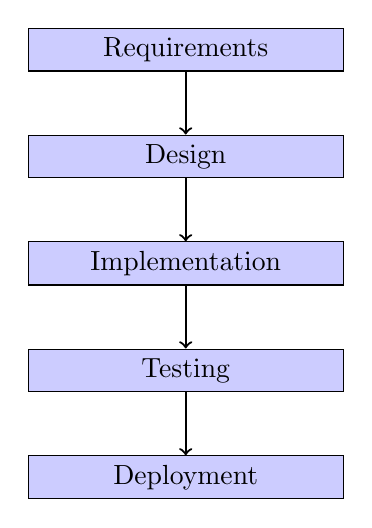
\begin{tikzpicture}[node distance=0.8cm]
    \node[draw, rectangle, fill=blue!20, minimum width=4cm] (req) {Requirements};
    \node[draw, rectangle, fill=blue!20, minimum width=4cm, below=of req] (des) {Design};
    \node[draw, rectangle, fill=blue!20, minimum width=4cm, below=of des] (imp) {Implementation};
    \node[draw, rectangle, fill=blue!20, minimum width=4cm, below=of imp] (test) {Testing};
    \node[draw, rectangle, fill=blue!20, minimum width=4cm, below=of test] (dep) {Deployment};

    \draw[->, thick] (req) -- (des);
    \draw[->, thick] (des) -- (imp);
    \draw[->, thick] (imp) -- (test);
    \draw[->, thick] (test) -- (dep);
\end{tikzpicture}
\end{center}

\textbf{Characteristics:}
\begin{itemize}
    \item Sequential, linear approach
    \item Each phase must complete before next begins
    \item Well-documented
\end{itemize}

\textbf{Best For:} Projects with well-defined, stable requirements

\textbf{Drawbacks:} Inflexible, late testing, difficult to accommodate changes

\subsection{Agile Model}

\textbf{Characteristics:}
\begin{itemize}
    \item Iterative and incremental
    \item Frequent deliveries (sprints)
    \item Embraces change
    \item Customer collaboration
    \item Working software over documentation
\end{itemize}

\textbf{Popular Frameworks:}
\begin{enumerate}
    \item \textbf{Scrum:} Sprint-based with defined roles
    \item \textbf{Kanban:} Visual workflow management
    \item \textbf{XP:} Extreme Programming with pair programming
\end{enumerate}

\textbf{Best For:} Projects with evolving requirements, need for flexibility

\subsection{V-Model}

\textbf{Characteristics:}
\begin{itemize}
    \item Each development phase has corresponding testing phase
    \item Verification and validation at each stage
    \item Testing planned in parallel with development
\end{itemize}

\textbf{Best For:} Projects requiring high reliability (medical, aerospace)

\subsection{Spiral Model}

\textbf{Characteristics:}
\begin{itemize}
    \item Risk-driven approach
    \item Combines iterative and waterfall
    \item Four phases repeated: Planning, Risk Analysis, Engineering, Evaluation
\end{itemize}

\textbf{Best For:} Large, complex, high-risk projects

\section{Choosing the Right Model}

\begin{tabular}{|l|l|}
\hline
\textbf{Scenario} & \textbf{Recommended Model} \\
\hline
Clear, fixed requirements & Waterfall \\
\hline
Evolving requirements & Agile \\
\hline
High-risk project & Spiral \\
\hline
Safety-critical system & V-Model \\
\hline
Quick prototype needed & Agile/Prototype \\
\hline
\end{tabular}

\section{SDLC in Your Project}

For your student projects, we recommend a \textbf{simplified Agile approach}:

\begin{enumerate}
    \item \textbf{Week 1-2:} Planning and Requirements
    \item \textbf{Week 3:} Design
    \item \textbf{Week 4-6:} Sprint 1 (Core features)
    \item \textbf{Week 7-9:} Sprint 2 (Additional features)
    \item \textbf{Week 10-11:} Sprint 3 (Polish and testing)
    \item \textbf{Week 12:} Deployment and Presentation
\end{enumerate}

\section{Summary}

\begin{itemize}
    \item SDLC provides a structured approach to software development
    \item Seven phases: Planning, Requirements, Design, Implementation, Testing, Deployment, Maintenance
    \item Different models suit different project types
    \item Agile is popular for modern software development
    \item Documentation is crucial throughout the process
\end{itemize}

\section{Discussion Questions}

\begin{enumerate}
    \item What SDLC model would you choose for a mobile app with unclear requirements?
    \item Why is the requirements phase so important?
    \item What happens if you skip the design phase?
    \item How does Agile handle changing requirements differently than Waterfall?
\end{enumerate}

\end{document}
